\documentclass[border=8pt]{standalone}
% Shared preamble for IronClaw thesis figures (standalone TikZ).
\renewcommand{\familydefault}{\sfdefault}
\usepackage{tikz}
\usetikzlibrary{arrows.meta,positioning,calc,fit,backgrounds,shapes.geometric,shapes.misc}

% IronClaw palette (matches slides.tex)
\definecolor{IronDark}{HTML}{1A2B3C}
\definecolor{IronBlue}{HTML}{2E86AB}
\definecolor{IronTeal}{HTML}{06A77D}
\definecolor{IronOrange}{HTML}{F18F01}
\definecolor{IronRed}{HTML}{C73E1D}
\definecolor{IronLight}{HTML}{F4F7F9}
\definecolor{IronGray}{HTML}{5D6D7E}

\tikzset{
  figtitle/.style={font=\large\bfseries\color{IronDark}, align=center},
  hostbox/.style={draw=IronBlue, rounded corners=5pt, fill=IronBlue!8,
                  line width=1pt, align=center, font=\small\color{white}},
  hostfill/.style={draw=IronBlue, rounded corners=4pt, fill=IronBlue,
                   line width=0.8pt, align=center, font=\small\color{white},
                   text width=3.1cm, minimum height=0.85cm},
  guestfill/.style={draw=IronOrange, rounded corners=4pt, fill=IronOrange!85,
                    line width=0.8pt, align=center, font=\small\color{white},
                    text width=3.1cm, minimum height=0.85cm},
  guestsoft/.style={draw=IronOrange, rounded corners=4pt, fill=IronOrange!25,
                    line width=0.8pt, align=center, font=\small\color{IronDark},
                    text width=3.1cm, minimum height=0.75cm},
  arrow/.style={-{Latex[length=2.6mm,width=2mm]}, line width=0.9pt, IronDark},
  biarrow/.style={{Latex[length=2.6mm,width=2mm]}-{Latex[length=2.6mm,width=2mm]},
                  line width=0.9pt, IronDark},
  note/.style={font=\footnotesize\color{IronGray}, align=center},
}

\begin{document}
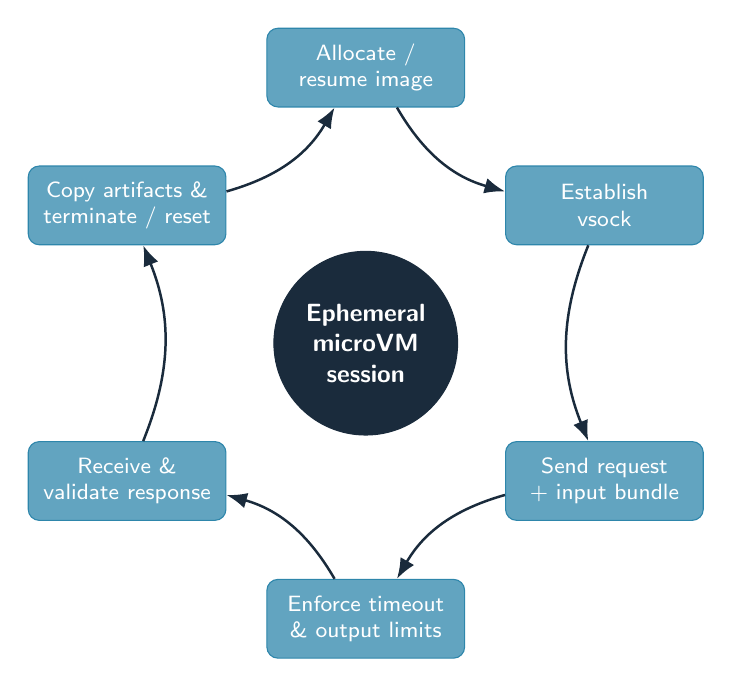
\begin{tikzpicture}
  \tikzset{
    stage/.style={draw=IronBlue, fill=IronBlue!75, text=white, rounded corners=4pt,
                  align=center, font=\footnotesize, text width=2.3cm,
                  minimum height=1.0cm, inner sep=3pt},
  }

  \def\R{3.5}
  \node[stage] (n1) at (90:\R)  {Allocate /\\resume image};
  \node[stage] (n2) at (30:\R)  {Establish\\vsock};
  \node[stage] (n3) at (-30:\R) {Send request\\+ input bundle};
  \node[stage] (n4) at (-90:\R) {Enforce timeout\\\& output limits};
  \node[stage] (n5) at (-150:\R){Receive \&\\validate response};
  \node[stage] (n6) at (150:\R) {Copy artifacts \&\\terminate / reset};

  \node[circle, draw=IronDark, fill=IronDark, text=white, align=center,
        font=\small\bfseries, text width=1.9cm, inner sep=2pt] (core) at (0,0)
        {Ephemeral microVM session};

  % clockwise arrows bowing outward, clear of node text
  \draw[arrow] (n1) to[bend right=22] (n2);
  \draw[arrow] (n2) to[bend right=22] (n3);
  \draw[arrow] (n3) to[bend right=22] (n4);
  \draw[arrow] (n4) to[bend right=22] (n5);
  \draw[arrow] (n5) to[bend right=22] (n6);
  \draw[arrow] (n6) to[bend right=22] (n1);

\end{tikzpicture}
\end{document}
